\documentclass[citation\_needed]{subfiles}
\begin{document}

Le corpus Quaero \citep{galibert2011structured} est un corpus d'oral transcrit constitué à partir de journaux télévisés Français dont une fiche récapitulative est donnée dans la figure\ \ref{tab:quaero-recap-card}. Une vision globale du corpus est donnée dans les tableaux de la figure \ref{fig:quaero-nombres}. La spécificité des entités nommées Quaero est qu'elle distingue deux types d'entités : les \emph{composants} et les \emph{types} (que nous appellerons \emph{entité} par soucis de clarté). Les \emph{entités} suivent la définition classique des entités nommées : elles peuvent être des lieux, personnes, organisations, montants, etc... Les \emph{composants}, comme leur nom l'indique, sont les différentes parties qui composent une entité. Par exemple, une personne a un prénom et/ou un nom,  une date absolue a potentiellement une année, un mois, un jour, etc... Cela signifie qu'un \emph{composant} ne peut pas être au plus haut niveau d'un arbre d'analyse en entités nommées. L'ensemble des \emph{composants} et des \emph{entités} est donné dans la figure\ \ref{fig:quaero-components-entities}.

\begin{table}[ht!]
\centering
\begin{tabular}{|p{0.21\linewidth}|p{0.21\linewidth}|p{0.21\linewidth}|p{0.21\linewidth}|}
\hline
\multicolumn{4}{|c|}{\textbf{corpus Quaero}} \\
\hline
\multicolumn{2}{|c|}{\textbf{général}} & \multicolumn{2}{c|}{\textbf{annotations}} \\
\hline
\textbf{type de texte} & journalistique,\newline divertissement & \textbf{niveaux\newline d'analyse} & $\emptyset$ \\
\hline
\textbf{unités d'analyse} & tour de parole & \textbf{structuration} & hiérarchique,\newline arborescente \\
\hline
\textbf{volume\newline texte brut} & 6.97 Mo & \textbf{types\newline d'entités} & 67 \\
\hline
\textbf{format} & pseudo-xml (annotations intégrées) & \textbf{entités\newline inconnues} & 37.73\% \\
\hline
\textbf{langue(s)} & Français & \textbf{$\kappa$} & 0.82607* \\
\hline
\end{tabular}
\scriptsize{\\ *évalué en considérant l'ensemble des entités annotées par au moins un annotateur.}
\caption{Fiche récapitulative du corpus FTB annoté EN}
\label{tab:quaero-recap-card}
\end{table}

La tâche de REN de Quaero est complexe pour de multiples raisons. La première étant qu'il s'agit d'un corpus d'oral transcrit, ce qui induit quelques problèmes connus : les marqueurs de discours, la grammaire non standard, et les problèmes de transcription. Les entités nommées Quaero sont également très variées et couvrantes, de nombreux noms communs étant annotés. Il existe nombreux \emph{composants transversaux} (cf figure\ \ref{fig:quaero-components-entities}), souvent polysémiques et/ou très contextuels (quelques \emph{composants}, comme \emph{qualifier}, n'apparaissent jamais de manière isolée). Une autre difficulté du Quaero est un grand déséquilibre entre les distributions des entités : \emph{amount} et ses composants \emph{val} et \emph{object} représentent 54\% du nombre total d'annotations.

\begin{figure}[ht!]
    \centering
    \begin{tabular}{|lc|c|c|}
    \cline{3-4}
    \multicolumn{2}{c|}{}            & entrainement & test \\
    \hline
    \multicolumn{2}{|l|}{documents}  & 188          & 18 \\
    \multicolumn{2}{|l|}{tokens}     & 1,291,225    & 108,010 \\
    \hline
    \multirow{2}{*}{composants} & v1 & 146,405      & 8,902 \\
                                & v2 & 255,498      & 13,612 \\
    \hline
    \multirow{2}{*}{entités}    & v1 & 113,885      & 5,523 \\
                                & v2 & 161,984      & 8,399 \\
    \hline
    \end{tabular}
    \caption{Statistics on the Quaero Train and Test Sets}
    \label{fig:quaero-nombres}
\end{figure}

\begin{figure}[ht!]
\begin{minipage}{0.49\linewidth}
    \centering
    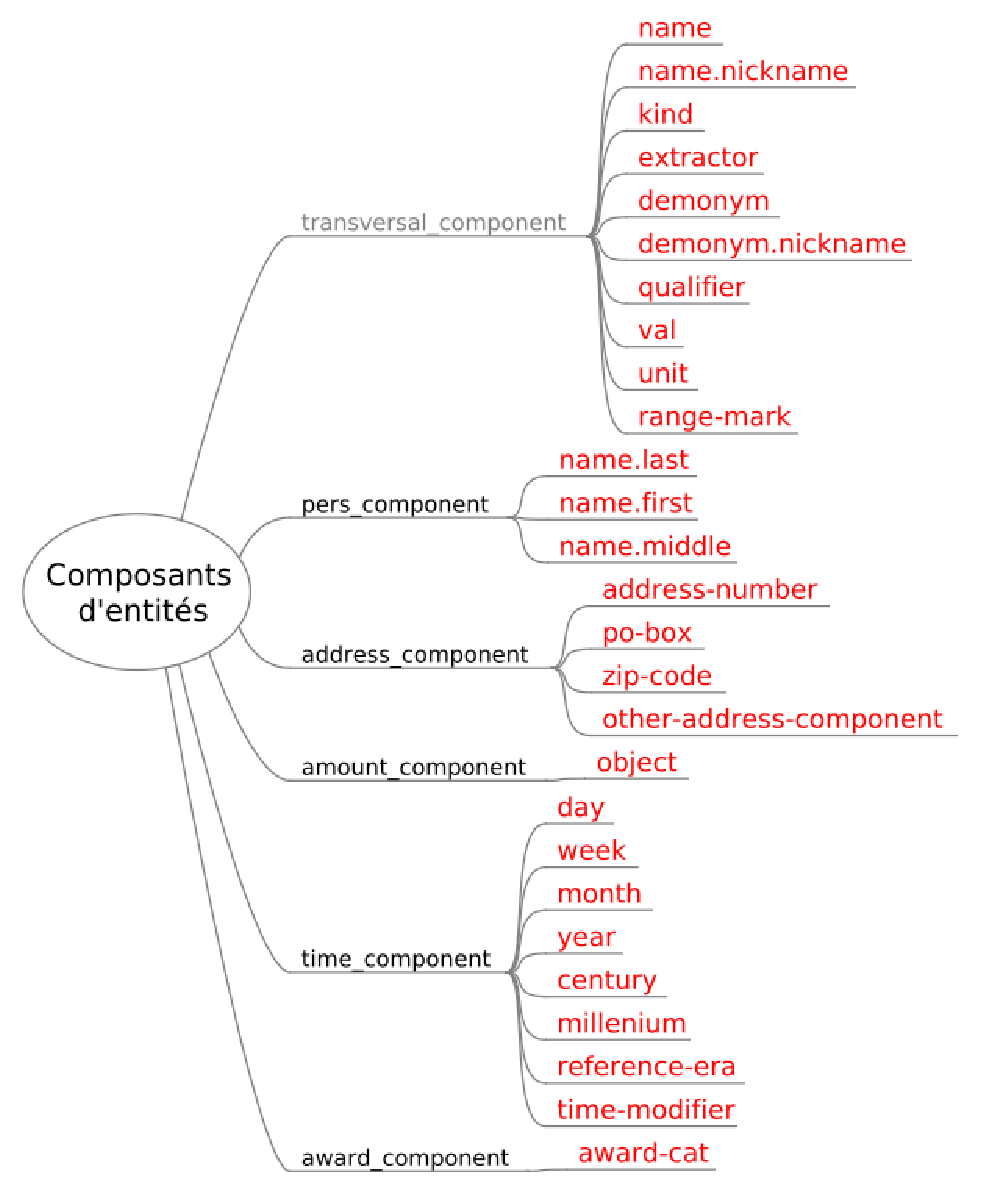
\includegraphics[scale=0.5]{images/quaero/annotation_guide-components}
\end{minipage}
\begin{minipage}{0.49\linewidth}
    \centering
   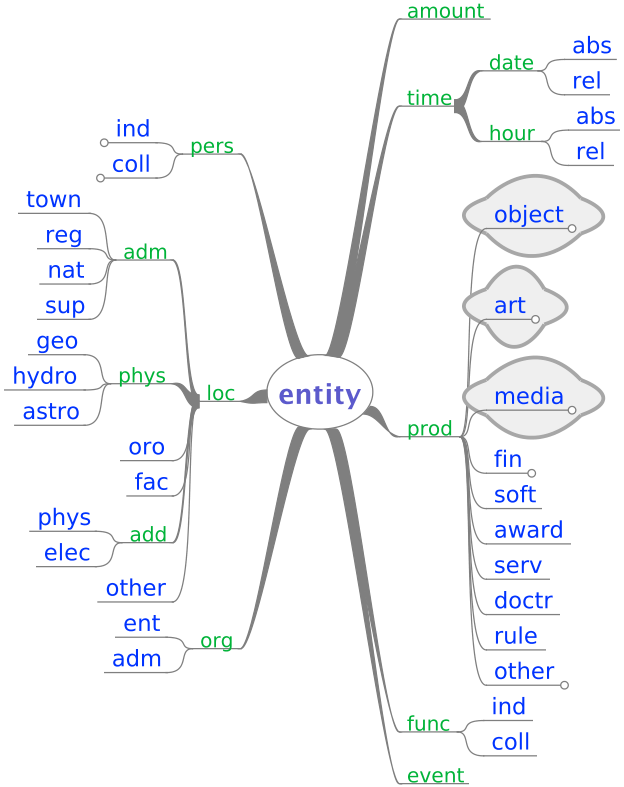
\includegraphics[scale=0.45]{images/quaero/annotation_guide-entities}
\end{minipage}
\caption{Les \emph{composants} et \emph{types} de Quaero}
\label{fig:quaero-components-entities}
\end{figure}

Quelques différences entre Quaero v1 et v2 sont données dans la figure \ref{fig:Quaerov1-vs-v2}. Parmi les plus notables est la disparition des sous-types d'organisations, c'est-à-dire \emph{org.ent} (entreprises), \emph{org.adm} (organisations) et \emph{org.other} (autres organisations), remplacées par \emph{org.ind} (organisation individuelle) et \emph{org.coll} (collection d'organisations). Certains composants \emph{kind} ont été redéfinis en \emph{func} (fonction), ce changement ayant pour conséquence la disparition des types \emph{func.ind} et \emph{func.coll}. Certains changements vont de pair avec d'autres précédemment cités : dans la v1, \emph{fonction} et \emph{personne} étaient deux différents types d'entité, alors qu'en v2 l'étendue d'une personne a été allongée pour intégrer sa fonction si présente. Ce changement fait écho au changement de certains \emph{kind} en \emph{func}.

\begin{figure}
\centering
\begin{tabular}{cccccccc}
\multirow{2}{*}{Quaero v1$\left\{\vphantom{\begin{tabular}{c}.\\.\end{tabular}}\right.$} &    & \multicolumn{4}{c}{\cellcolor{red}func.ind}                                & \multicolumn{2}{c}{\cellcolor{yellow!75}pers.ind}\\
                           &    & \cellcolor{blue!50}kind     &     & \multicolumn{2}{c}{\cellcolor{green!75}name} & \cellcolor{red!33}name.first & \cellcolor{red!66}name.last\\
                           & le & président                   & du  & Burkina & Faso                               & Blaise     & Compaoré\\
\multirow{2}{*}{Quaero v2$\left\{\vphantom{\begin{tabular}{c}.\\.\end{tabular}}\right.$} &    & \cellcolor{teal!66}function &     & \multicolumn{2}{c}{\cellcolor{green!75}name} & \cellcolor{red!33}name.first & \cellcolor{red!66}name.last\\
                           &    & \multicolumn{6}{c}{\cellcolor{yellow!75}pers.ind}\\
\end{tabular}

~\\~\\

\begin{tabular}{cccccccc}
\multirow{2}{*}{Quaero v1$\left\{\vphantom{\begin{tabular}{c}.\\.\end{tabular}}\right.$} & & \cellcolor{blue!50}org.adm & [...] & & & & \cellcolor{teal!66}org.ent \\
 & & \cellcolor{red!66}name & [...] & & & & \cellcolor{red!66}name \\
 & l' & État & [...] & à & aider & la & compagnie \\
\multirow{2}{*}{Quaero v2$\left\{\vphantom{\begin{tabular}{c}.\\.\end{tabular}}\right.$}  & & \cellcolor{red!66}name & [...] & & & & \cellcolor{red!66}name \\
& & \cellcolor{green!66}org.ind & [...] & & & & \cellcolor{green!66}org.ind \\
\end{tabular}
\caption{quelques différences entre Quaero v1 et v2}
\label{fig:Quaerov1-vs-v2}
\end{figure}

Quaero offre un grand nombre d'annotations de natures très variées, nombre d'entités étant des groupes nominaux ou des noms propres. C'est par exemple le cas des \emph{amount} (montant), dont deux exemples sont «~deux indencies~» ou «~des historiens~», mais qui ne comprennent en revanche pas les résultats sportif ou le langage administratif (assertion 22 du guide d'annotation Quaero). La nature générique de certaines entités les rend parfois difficile à appréhender, même humainement (dans certains cas de figure, certains types ou composants ne sont pas obligatoires).

Bien que la plupart des entités Quaero soient de profondeur 2, il n'y a pas de limite théorique à la profondeur que peut avoir une entité Quaero : la plus profonde que nous ayons trouvée dans le corpus a une profondeur de 9 et est donnée dans la figure \ref{fig:quaero-deepest}.

\begin{figure}
\scriptsize
\center
\begin{forest}
[\textcolor{blue}{\textbf{amount}}
    [\textcolor{red}{\textbf{extractor}} [un]]
    [des]
    [\textcolor{red}{\textbf{object}}
        [\textcolor{blue}{\textbf{pers.coll}}
            [\textcolor{red}{\textbf{qualifier}} [principaux]]
            [\textcolor{red}{\textbf{func}} [chefs]]
            [\textcolor{red}{\textbf{qualifier}} [militaires]]
            [du]
            [\textcolor{blue}{\textbf{org.ind}}
                [\textcolor{red}{\textbf{name}}
                    [\textcolor{red}{\textbf{kind}} [mouvement]]
                    [\textcolor{red}{\textbf{qualifier}} [patriotique]]
                    de
                    [\textcolor{blue}{\textbf{loc.adm.nat}}
                        [\textcolor{red}{\textbf{name}}
                            [\textcolor{blue}{\textbf{loc.phys.geo}}
                                [\textcolor{red}{\textbf{kind}} [côte]]
                                [d']
                                [ivoire]
                            ]
                        ]
                    ]
                ]
            ]
        ]
    ]
]
\end{forest}
\caption{l'arbre le plus profond de Quaero}
\label{fig:quaero-deepest}
\end{figure}

\end{document}